\documentclass{article}

\usepackage{inputenc}
\usepackage{csquotes}
\usepackage[a4paper, total={6in, 10in}]{geometry}
\usepackage{hyperref}
\usepackage{amsmath,amssymb}
\usepackage{graphicx}
\usepackage{indentfirst}
\usepackage{caption}
\usepackage{subcaption}
\usepackage[
singlelinecheck=false, % <-- important 
justification = centering
]{caption}
\usepackage{float}
\usepackage{booktabs}
\begin{document}

\begin{table}[h!] \centering
   \caption{Main table}
   {
\def\sym#1{\ifmmode^{#1}\else\(^{#1}\)\fi}
\begin{tabular}{l*{3}{c}}
\hline\hline
          &\multicolumn{1}{c}{(1)}&\multicolumn{1}{c}{(2)}&\multicolumn{1}{c}{(3)}\\
          &\multicolumn{1}{c}{D.ln\_med\_rent\_psqft}&\multicolumn{1}{c}{D.ln\_med\_rent\_psqft}&\multicolumn{1}{c}{D.ln\_med\_rent\_psqft}\\
\hline
D.ln\_mw   &   0.0257\sym{*}  &   0.0253\sym{**} &   0.0250\sym{**} \\
          & (0.0128)         & (0.0121)         & (0.0117)         \\
\hline
Zipcode-specifc linear trend&       No         &      Yes         &      Yes         \\
Zipcode-specific linear and square trend&       No         &       No         &      Yes         \\
R-squared &                  &                  &                  \\
Observations&    0.022         &    0.023         &    0.026         \\
N         &   113363         &   113363         &   113363         \\
\hline\hline
\end{tabular}
}

\end{table}

\begin{table}[h!] \centering
	\caption{Polynomial trends}
	{
\def\sym#1{\ifmmode^{#1}\else\(^{#1}\)\fi}
\begin{tabular}{l*{6}{c}}
\hline\hline
          &\multicolumn{1}{c}{(1)}         &\multicolumn{1}{c}{(2)}         &\multicolumn{1}{c}{(3)}         &\multicolumn{1}{c}{(4)}         &\multicolumn{1}{c}{(5)}         &\multicolumn{1}{c}{(6)}         \\
\hline
$\Delta \ln \underline{w}_{ict}$&   0.0260\sym{**} &   0.0257\sym{**} &   0.0255\sym{**} &   0.0258\sym{**} &   0.0248\sym{**} &   0.0242\sym{**} \\
          & (0.0128)         & (0.0120)         & (0.0117)         & (0.0124)         & (0.0116)         & (0.0111)         \\
\hline
\vspace{-2mm}&                  &                  &                  &                  &                  &                  \\
Zipcode-specifc linear trend&       No         &      Yes         &      Yes         &       No         &      Yes         &      Yes         \\
Zipcode-specific quadratic trend&       No         &       No         &      Yes         &       No         &       No         &      Yes         \\
Local economy controls&       No         &       No         &       No         &      Yes         &      Yes         &      Yes         \\
R-squared &    0.022         &    0.024         &    0.026         &    0.022         &    0.024         &    0.027         \\
Observations&  112,232         &  112,232         &  112,232         &  107,814         &  107,814         &  107,814         \\
\hline\hline
\end{tabular}
}

\end{table}

\clearpage
\begin{table}[h!]\centering
	\caption{Dynamic models}
	{
\def\sym#1{\ifmmode^{#1}\else\(^{#1}\)\fi}
\begin{tabular}{l*{5}{c}}
\hline\hline
          &\multicolumn{1}{c}{(1)}         &\multicolumn{1}{c}{(2)}         &\multicolumn{1}{c}{(3)}         &\multicolumn{1}{c}{(4)}         &\multicolumn{1}{c}{(5)}         \\
\hline
$\Delta \ln \underline{w}_{ic,t-5}$&  -0.0148         &  -0.0144         &  -0.0144         &  -0.0146         &  -0.0144         \\
          & (0.0090)         & (0.0089)         & (0.0089)         & (0.0090)         & (0.0089)         \\
[1em]
$\Delta \ln \underline{w}_{ic,t-4}$&  -0.0024         &  -0.0019         &  -0.0020         &  -0.0022         &  -0.0019         \\
          & (0.0116)         & (0.0116)         & (0.0115)         & (0.0116)         & (0.0115)         \\
[1em]
$\Delta \ln \underline{w}_{ic,t-3}$&   0.0011         &   0.0005         &   0.0007         &   0.0004         &  -0.0002         \\
          & (0.0092)         & (0.0094)         & (0.0092)         & (0.0091)         & (0.0092)         \\
[1em]
$\Delta \ln \underline{w}_{ic,t-2}$&   0.0060         &   0.0063         &   0.0062         &   0.0060         &   0.0064         \\
          & (0.0116)         & (0.0118)         & (0.0116)         & (0.0115)         & (0.0117)         \\
[1em]
$\Delta \ln \underline{w}_{ic,t-1}$&  -0.0002         &  -0.0004         &  -0.0005         &   0.0000         &  -0.0005         \\
          & (0.0123)         & (0.0123)         & (0.0124)         & (0.0122)         & (0.0123)         \\
[1em]
$\Delta \ln \underline{w}_{ic,t}$&   0.0271\sym{**} &   0.0257\sym{**} &   0.0259\sym{**} &   0.0269\sym{**} &   0.0259\sym{**} \\
          & (0.0126)         & (0.0123)         & (0.0124)         & (0.0126)         & (0.0124)         \\
[1em]
$\Delta \ln \underline{w}_{ic,t+1}$&   0.0136\sym{*}  &   0.0146\sym{**} &   0.0142\sym{*}  &   0.0135\sym{*}  &   0.0146\sym{*}  \\
          & (0.0072)         & (0.0072)         & (0.0072)         & (0.0072)         & (0.0072)         \\
[1em]
$\Delta \ln \underline{w}_{ic,t+2}$&  -0.0070         &  -0.0066         &  -0.0064         &  -0.0068         &  -0.0064         \\
          & (0.0133)         & (0.0133)         & (0.0132)         & (0.0133)         & (0.0132)         \\
[1em]
$\Delta \ln \underline{w}_{ic,t+3}$&   0.0036         &   0.0045         &   0.0047         &   0.0031         &   0.0040         \\
          & (0.0081)         & (0.0078)         & (0.0078)         & (0.0079)         & (0.0077)         \\
[1em]
$\Delta \ln \underline{w}_{ic,t+4}$&   0.0108         &   0.0093         &   0.0104         &   0.0107         &   0.0096         \\
          & (0.0069)         & (0.0066)         & (0.0064)         & (0.0069)         & (0.0065)         \\
[1em]
$\Delta \ln \underline{w}_{ic,t+5}$&   0.0086         &   0.0095         &   0.0099         &   0.0088         &   0.0099         \\
          & (0.0069)         & (0.0065)         & (0.0065)         & (0.0067)         & (0.0065)         \\
\hline
\vspace{-2mm}&                  &                  &                  &                  &                  \\
Cumulative effect&    0.057         &0.057\sym{*}         &0.059\sym{*}         &    0.056         &0.058\sym{*}         \\
          &  (0.035)         &  (0.034)         &  (0.034)         &  (0.034)         &  (0.034)         \\
\hline    &                  &                  &                  &                  &                  \\
P-value no pretrends&    0.568         &    0.612         &    0.599         &    0.594         &    0.629         \\
Wage controls&       No         &      Yes         &       No         &       No         &      Yes         \\
Employment controls&       No         &       No         &      Yes         &       No         &      Yes         \\
Establishment-count controls&       No         &       No         &       No         &      Yes         &      Yes         \\
R-squared &    0.022         &    0.022         &    0.022         &    0.022         &    0.022         \\
Observations&  106,446         &  105,463         &  105,463         &  106,160         &  105,463         \\
\hline\hline
\end{tabular}
}

\end{table}

\clearpage
\begin{table}[h!]\centering
	\caption{Horse race models}
	\resizebox{\textwidth}{!}{
		{
\def\sym#1{\ifmmode^{#1}\else\(^{#1}\)\fi}
\begin{tabular}{l*{8}{c}}
\hline\hline
          &\multicolumn{1}{c}{(1)}&\multicolumn{1}{c}{(2)}&\multicolumn{1}{c}{(3)}&\multicolumn{1}{c}{(4)}&\multicolumn{1}{c}{(5)}&\multicolumn{1}{c}{(6)}&\multicolumn{1}{c}{(7)}&\multicolumn{1}{c}{(8)}\\
          &\multicolumn{1}{c}{DiD}&\multicolumn{1}{c}{Distributed leads and lags}&\multicolumn{1}{c}{Distributed Lags}&\multicolumn{1}{c}{AB distributed leads and lags}&\multicolumn{1}{c}{AB distributed lags}&\multicolumn{1}{c}{est6}&\multicolumn{1}{c}{est7}&\multicolumn{1}{c}{est8}\\
\hline
\Delta ln(MW)_{t-5}&                  &  -0.0146         &                  &  -0.0159         &  -0.0134         &                  &  -0.0167         &                  \\
          &                  &(0.00910)         &                  &(0.00991)         &(0.00910)         &                  & (0.0155)         &                  \\
[1em]
\Delta ln(MW)_{t-4}&                  & -0.00232         &                  & -0.00576         &  0.00494         &                  & -0.00886         &                  \\
          &                  & (0.0116)         &                  & (0.0129)         & (0.0105)         &                  & (0.0347)         &                  \\
[1em]
\Delta ln(MW)_{t-3}&                  &  0.00137         &                  &  0.00100         &  0.00222         &                  & 0.000503         &                  \\
          &                  &(0.00931)         &                  & (0.0106)         &(0.00918)         &                  & (0.0152)         &                  \\
[1em]
\Delta ln(MW)_{t-2}&                  &  0.00608         &                  &  0.00625         &  0.00581         &                  &  0.00647         &                  \\
          &                  & (0.0115)         &                  & (0.0107)         & (0.0139)         &                  & (0.0102)         &                  \\
[1em]
\Delta ln(MW)_{t-1}&                  &-0.000280         &                  & -0.00141         & -0.00531         &                  &-0.000132         &                  \\
          &                  & (0.0123)         &                  &(0.00995)         & (0.0151)         &                  & (0.0154)         &                  \\
[1em]
\Delta ln(MW)_{t}&   0.0259\sym{*}  &   0.0270\sym{**} &   0.0261\sym{*}  &   0.0269\sym{**} &   0.0294\sym{*}  &   0.0288\sym{*}  &   0.0267\sym{**} &   0.0256\sym{**} \\
          & (0.0129)         & (0.0127)         & (0.0129)         & (0.0111)         & (0.0157)         & (0.0160)         & (0.0104)         & (0.0106)         \\
[1em]
\Delta ln(MW)_{t+1}&                  &   0.0136\sym{*}  &   0.0161\sym{**} &   0.0205\sym{**} & 0.000887         &  0.00401         &   0.0267         &   0.0304         \\
          &                  &(0.00715)         &(0.00750)         &(0.00860)         &(0.00733)         &(0.00788)         & (0.0514)         & (0.0536)         \\
[1em]
\Delta ln(MW)_{t+2}&                  & -0.00702         & -0.00673         & -0.00389         &  -0.0131         &  -0.0142         & -0.00102         &  0.00170         \\
          &                  & (0.0133)         & (0.0125)         & (0.0138)         & (0.0128)         & (0.0120)         & (0.0286)         & (0.0354)         \\
[1em]
\Delta ln(MW)_{t+3}&                  &  0.00364         &  0.00392         &  0.00211         &  0.00651         &  0.00692         & 0.000616         & 0.000316         \\
          &                  &(0.00808)         &(0.00799)         &(0.00972)         &(0.00798)         &(0.00764)         & (0.0158)         & (0.0173)         \\
[1em]
\Delta ln(MW)_{t+4}&                  &   0.0108         &   0.0105         &   0.0112         &  0.00897         &  0.00850         &   0.0120         &   0.0122         \\
          &                  &(0.00693)         &(0.00684)         &(0.00737)         &(0.00736)         &(0.00737)         & (0.0108)         & (0.0119)         \\
[1em]
\Delta ln(MW)_{t+5}&                  &  0.00862         &  0.00637         &   0.0102         &  0.00384         &  0.00163         &   0.0124         &   0.0112         \\
          &                  &(0.00686)         &(0.00675)         &(0.00655)         &(0.00878)         &(0.00870)         & (0.0160)         & (0.0174)         \\
[1em]
\Delta ln(y)_{t-1}&                  &                  &                  &   -0.240\sym{***}&    0.421\sym{***}&    0.436\sym{***}&   -0.451         &   -0.531         \\
          &                  &                  &                  &(0.00646)         & (0.0238)         & (0.0231)         &  (1.634)         &  (1.812)         \\
\hline
Observations& 1.12e+05         & 1.06e+05         & 1.12e+05         & 1.05e+05         & 1.04e+05         & 1.10e+05         & 1.05e+05         & 1.11e+05         \\
\hline\hline
\end{tabular}
}

	}
\end{table}

\clearpage
\begin{table}[h!]\centering
	\caption{External Validity and Sensitivity Robustness Checks}
	\label{tab:wgt_unbal_comparison}
	\resizebox{0.8\textwidth}{!}{
		{
\def\sym#1{\ifmmode^{#1}\else\(^{#1}\)\fi}
\begin{tabular}{l*{3}{c}}
\hline\hline
          &\multicolumn{1}{c}{(1)}&\multicolumn{1}{c}{(2)}&\multicolumn{1}{c}{(3)}\\
          &\multicolumn{1}{c}{Baseline}&\multicolumn{1}{c}{Reweighted}&\multicolumn{1}{c}{Unbalanced}\\
\hline
Static Effect&   0.0257\sym{**} &   0.0389\sym{***}&   0.0225\sym{*}  \\
          & (0.0124)         & (0.0131)         & (0.0115)         \\
\hline
\vspace{-2mm}&                  &                  &                  \\
Cumulative effect&0.0595\sym{*}         &0.0737\sym{*}         &0.0534\sym{*}         \\
          & (0.0343)         & (0.0428)         & (0.0297)         \\
Long-run effect&0.0602\sym{**}         &0.0687\sym{***}         &   0.0332         \\
          & (0.0234)         & (0.0243)         &  (0.024)         \\
\hline    &                  &                  &                  \\
Wage controls&      Yes         &      Yes         &      Yes         \\
Employment controls&      Yes         &      Yes         &      Yes         \\
Establishment-count controls&      Yes         &      Yes         &      Yes         \\
Observations (static model)&  107,781         &  107,781         &  182,608         \\
\hline\hline
\end{tabular}
}

	}
\end{table}

\clearpage
\begin{table}[h!]\centering
	\caption{Experienced Minimum Wage}
	\label{tab:base_expmw_comparison}
	\resizebox{0.8\textwidth}{!}{
		{
\def\sym#1{\ifmmode^{#1}\else\(^{#1}\)\fi}
\begin{tabular}{l*{2}{c}}
\hline\hline
          &\multicolumn{1}{c}{(1)}&\multicolumn{1}{c}{(2)}\\
          &\multicolumn{1}{c}{Baseline}&\multicolumn{1}{c}{\Delta \ln{Exp.MW}}\\
\hline
Static Effect&   0.0257\sym{**} &   0.0308\sym{**} \\
          & (0.0124)         & (0.0132)         \\
\hline
\vspace{-1mm}&                  &                  \\
Cumulative effect&0.058\sym{*}         &0.063\sym{*}         \\
          &  (0.034)         &  (0.037)         \\
\hline    &                  &                  \\
P-value no pretrends&    0.626         &    0.599         \\
Wage controls&      Yes         &      Yes         \\
Employment controls&      Yes         &      Yes         \\
Establishment-count controls&      Yes         &      Yes         \\
R-squared &    0.022         &    0.022         \\
Observations&  107,781         &  107,781         \\
\hline\hline
\end{tabular}
}

	}
\end{table}


%%%%%%%%%%%%%%%%%%%%%%%%%%%%%%%%%%%%%%%%%%%%%%%%%%%%%%%%%%%%%%%%%%%%%%%%%%%%%%%%%%%%
%%%%%%%                              FIGURES                                %%%%%%%%
%%%%%%%%%%%%%%%%%%%%%%%%%%%%%%%%%%%%%%%%%%%%%%%%%%%%%%%%%%%%%%%%%%%%%%%%%%%%%%%%%%%%

\clearpage
\begin{figure}[htb!]
	\caption{Dynamic model}
	\centering
	\begin{subfigure}[b]{0.8\textwidth}
		\caption{Coefficients}
		\includegraphics[width = \textwidth]
		{../../analysis/first_differences/output/fd_models_coeffs_w5.eps}
	\end{subfigure}
	\begin{subfigure}[b]{0.8\textwidth}
		\caption{Cumulative sum}
		\includegraphics[width = \textwidth]
		{../../analysis/first_differences/output/fd_models_cumsum.eps}
	\end{subfigure}
\end{figure}


\clearpage
\begin{figure}[htb!]
	\caption{Dynamic model: changing window}
	\centering
	\begin{subfigure}[b]{0.5\textwidth}
		\caption{$w=3$}
		\includegraphics[width = \textwidth]
		{../../analysis/first_differences/output/fd_models_coeffs_w3.eps}
	\end{subfigure}%
	\begin{subfigure}[b]{0.5\textwidth}
		\caption{$w=6$}
		\includegraphics[width = \textwidth]
		{../../analysis/first_differences/output/fd_models_coeffs_w6.eps}
	\end{subfigure}\\
	\begin{subfigure}[b]{0.5\textwidth}
		\caption{$w=9$}
		\includegraphics[width = \textwidth]
		{../../analysis/first_differences/output/fd_models_coeffs_w9.eps}
	\end{subfigure}
\end{figure}

\begin{figure} \centering
	\caption{Dynamic model: varying controls}
	\includegraphics[width = 0.8\textwidth]{../../analysis/first_differences/output/fd_models_control.eps}
\end{figure} 

\clearpage 
\begin{figure}[htb!]\centering
	\caption{Placebo Regression with Dependent Variable: (log) Number of for Sale Listings}
	\label{fig:placebo_nlist}
	\includegraphics[width = 0.8\textwidth]{../../analysis/first_differences_nlist/output/fd_placebo.eps}	
\end{figure}


\clearpage
\begin{figure}[htb!]\centering
	\caption{Comparison between Dynamic Baseline Model, Re weighted Model, and Unbalanced-panel Model}
	\label{fig:dynamic_wgt_unabl_comp}
	\begin{subfigure}[b]{\textwidth}
	\caption{Baseline-Re weighted Models}	
	\includegraphics[width = \textwidth]{../../analysis/first_differences_wgt/output/fd_model_comparison_wgt.eps}
	\end{subfigure}
	\quad
	\begin{subfigure}[b]{\textwidth}
	\caption{Baseline-Unbalanced Models}		
	\includegraphics[width = \textwidth]{../../analysis/first_differences_unbal/output/fd_model_comparison_unbal.eps}
	\end{subfigure}
\end{figure}


\clearpage 
\begin{figure}[htb!]\centering
	\caption{Effect of Minimum Wage on Rents by Quartiles of Low-income and Young Workers' share Distribution}
	\label{fig:static_qtl_lodes}
	\begin{subfigure}[b]{\textwidth}
		\caption{Workplace Distribution}
		\includegraphics[width = .8\textwidth]{../../analysis/first_differences_expmw/output/fd_static_heter_walall_29y_lowinc_ssh_st_qtl.eps}
	\end{subfigure}
	\begin{subfigure}[b]{\textwidth}
	\caption{Residential Distribution}
	\includegraphics[width = .8\textwidth]{../../analysis/first_differences_expmw/output/fd_static_heter_halall_29y_lowinc_ssh_st_qtl.eps}
	\end{subfigure}
\end{figure}

\clearpage 
\begin{figure}[htb!]\centering
	\caption{Effect of Minimum Wage on Rents by Quartiles of Low-income and Young Workers' share Distribution}
	\label{fig:static_qtl_lodes-2}
	\begin{subfigure}[b]{\textwidth}
		\caption{Workplace Distribution}
		\includegraphics[width = .8\textwidth]{../../analysis/first_differences_expmw/output/fd_static_heter_walall_29y_lowinc_zsh_st_qtl.eps}
	\end{subfigure}
	\begin{subfigure}[b]{\textwidth}
		\caption{Residential Distribution}
		\includegraphics[width = .8\textwidth]{../../analysis/first_differences_expmw/output/fd_static_heter_halall_29y_lowinc_zsh_st_qtl.eps}
	\end{subfigure}
\end{figure}

\clearpage 
\begin{figure}[htb!]\centering
	\caption{Comparison between Baseline Model and Model using Experienced Minimum Wage as main Explanatory Variable}
	\label{fig: dynamic_base_expmw_comp}
	\includegraphics[width = .8\textwidth]{../../analysis/first_differences_expmw/output/fd_model_comparison_expmw.eps}
\end{figure}


\clearpage
\begin{figure}
	\caption{Comparison Between Zillow Sample and Population Density in CBSAs}
	\begin{subfigure}[b]{\textwidth}\centering
		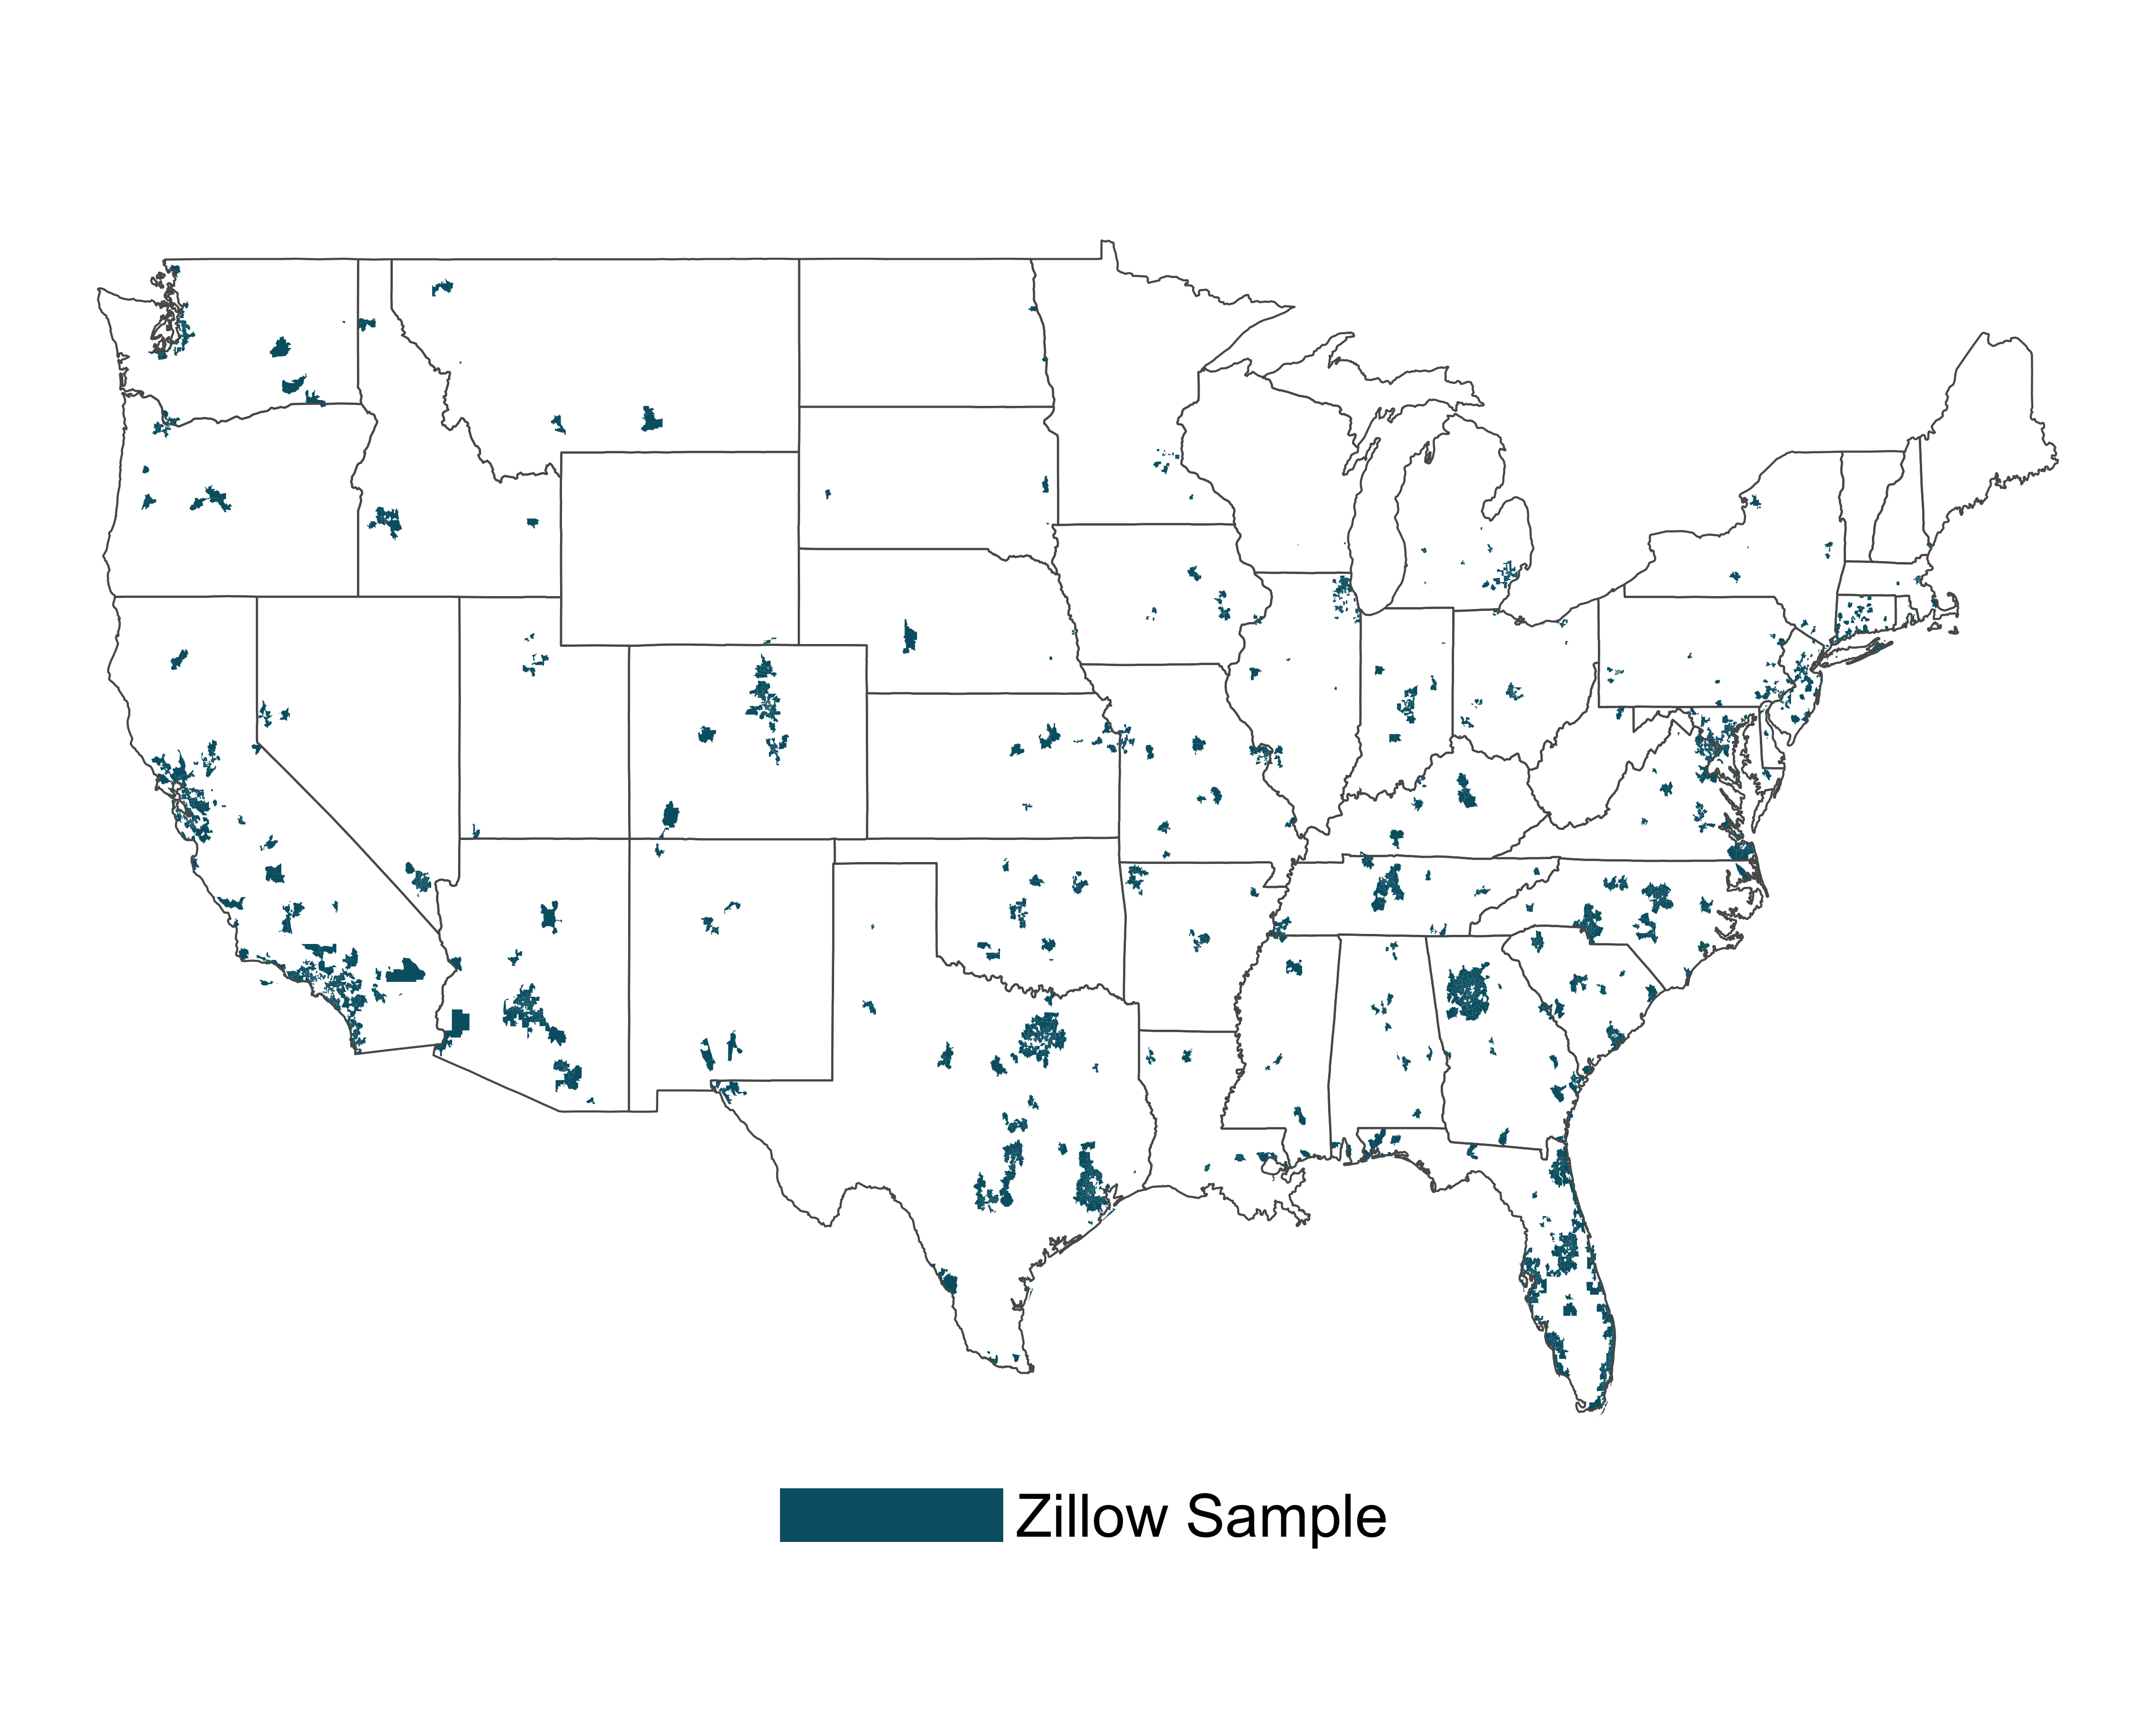
\includegraphics[width = .9\textwidth]{../../analysis/descriptive_maps/output/sample_map.png}
	\end{subfigure}
	\quad 
	\begin{subfigure}[b]{\textwidth}\centering
		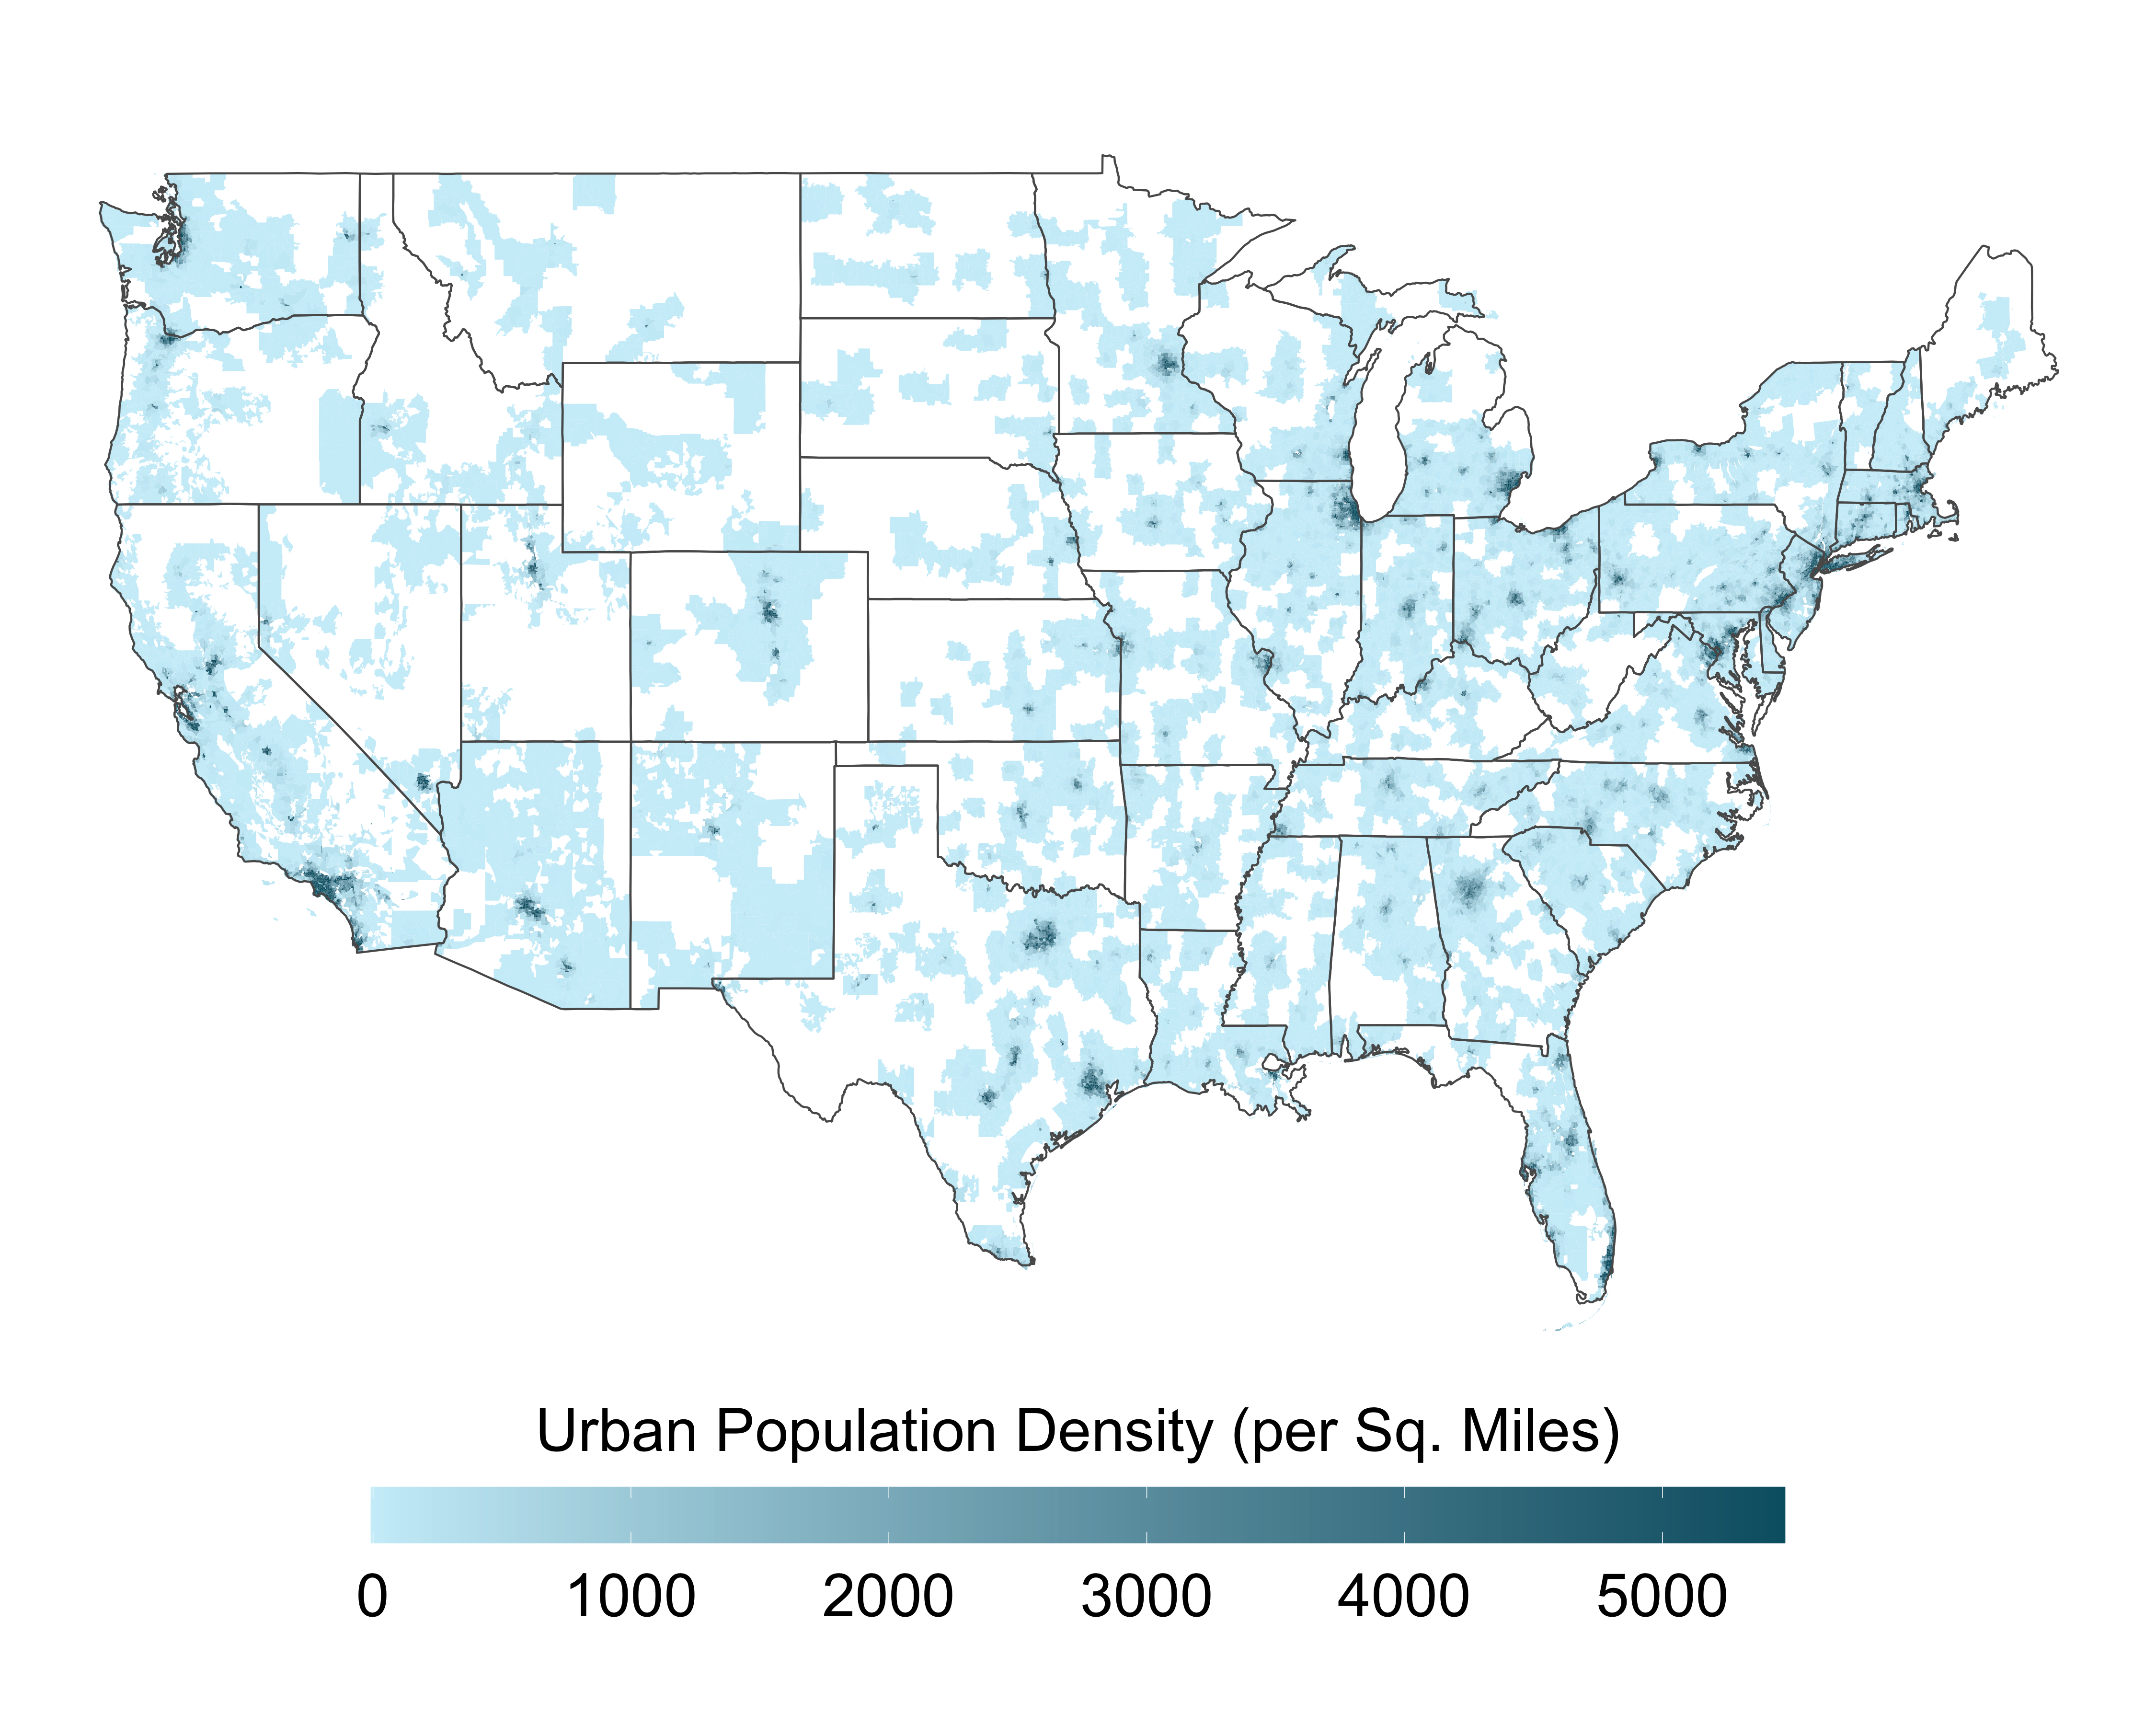
\includegraphics[width = .9\textwidth]{../../analysis/descriptive_maps/output/popurban_density_map.png}
	\end{subfigure}
\end{figure}


\clearpage
\begin{figure}\centering
	\captionsetup[subfigure]{justification=centering}
	\caption{Comparison Between Statutory and Experienced Minimum Wage Change for the Seattle MSA}
	\begin{subfigure}[b]{.8\textwidth}
		\centering
		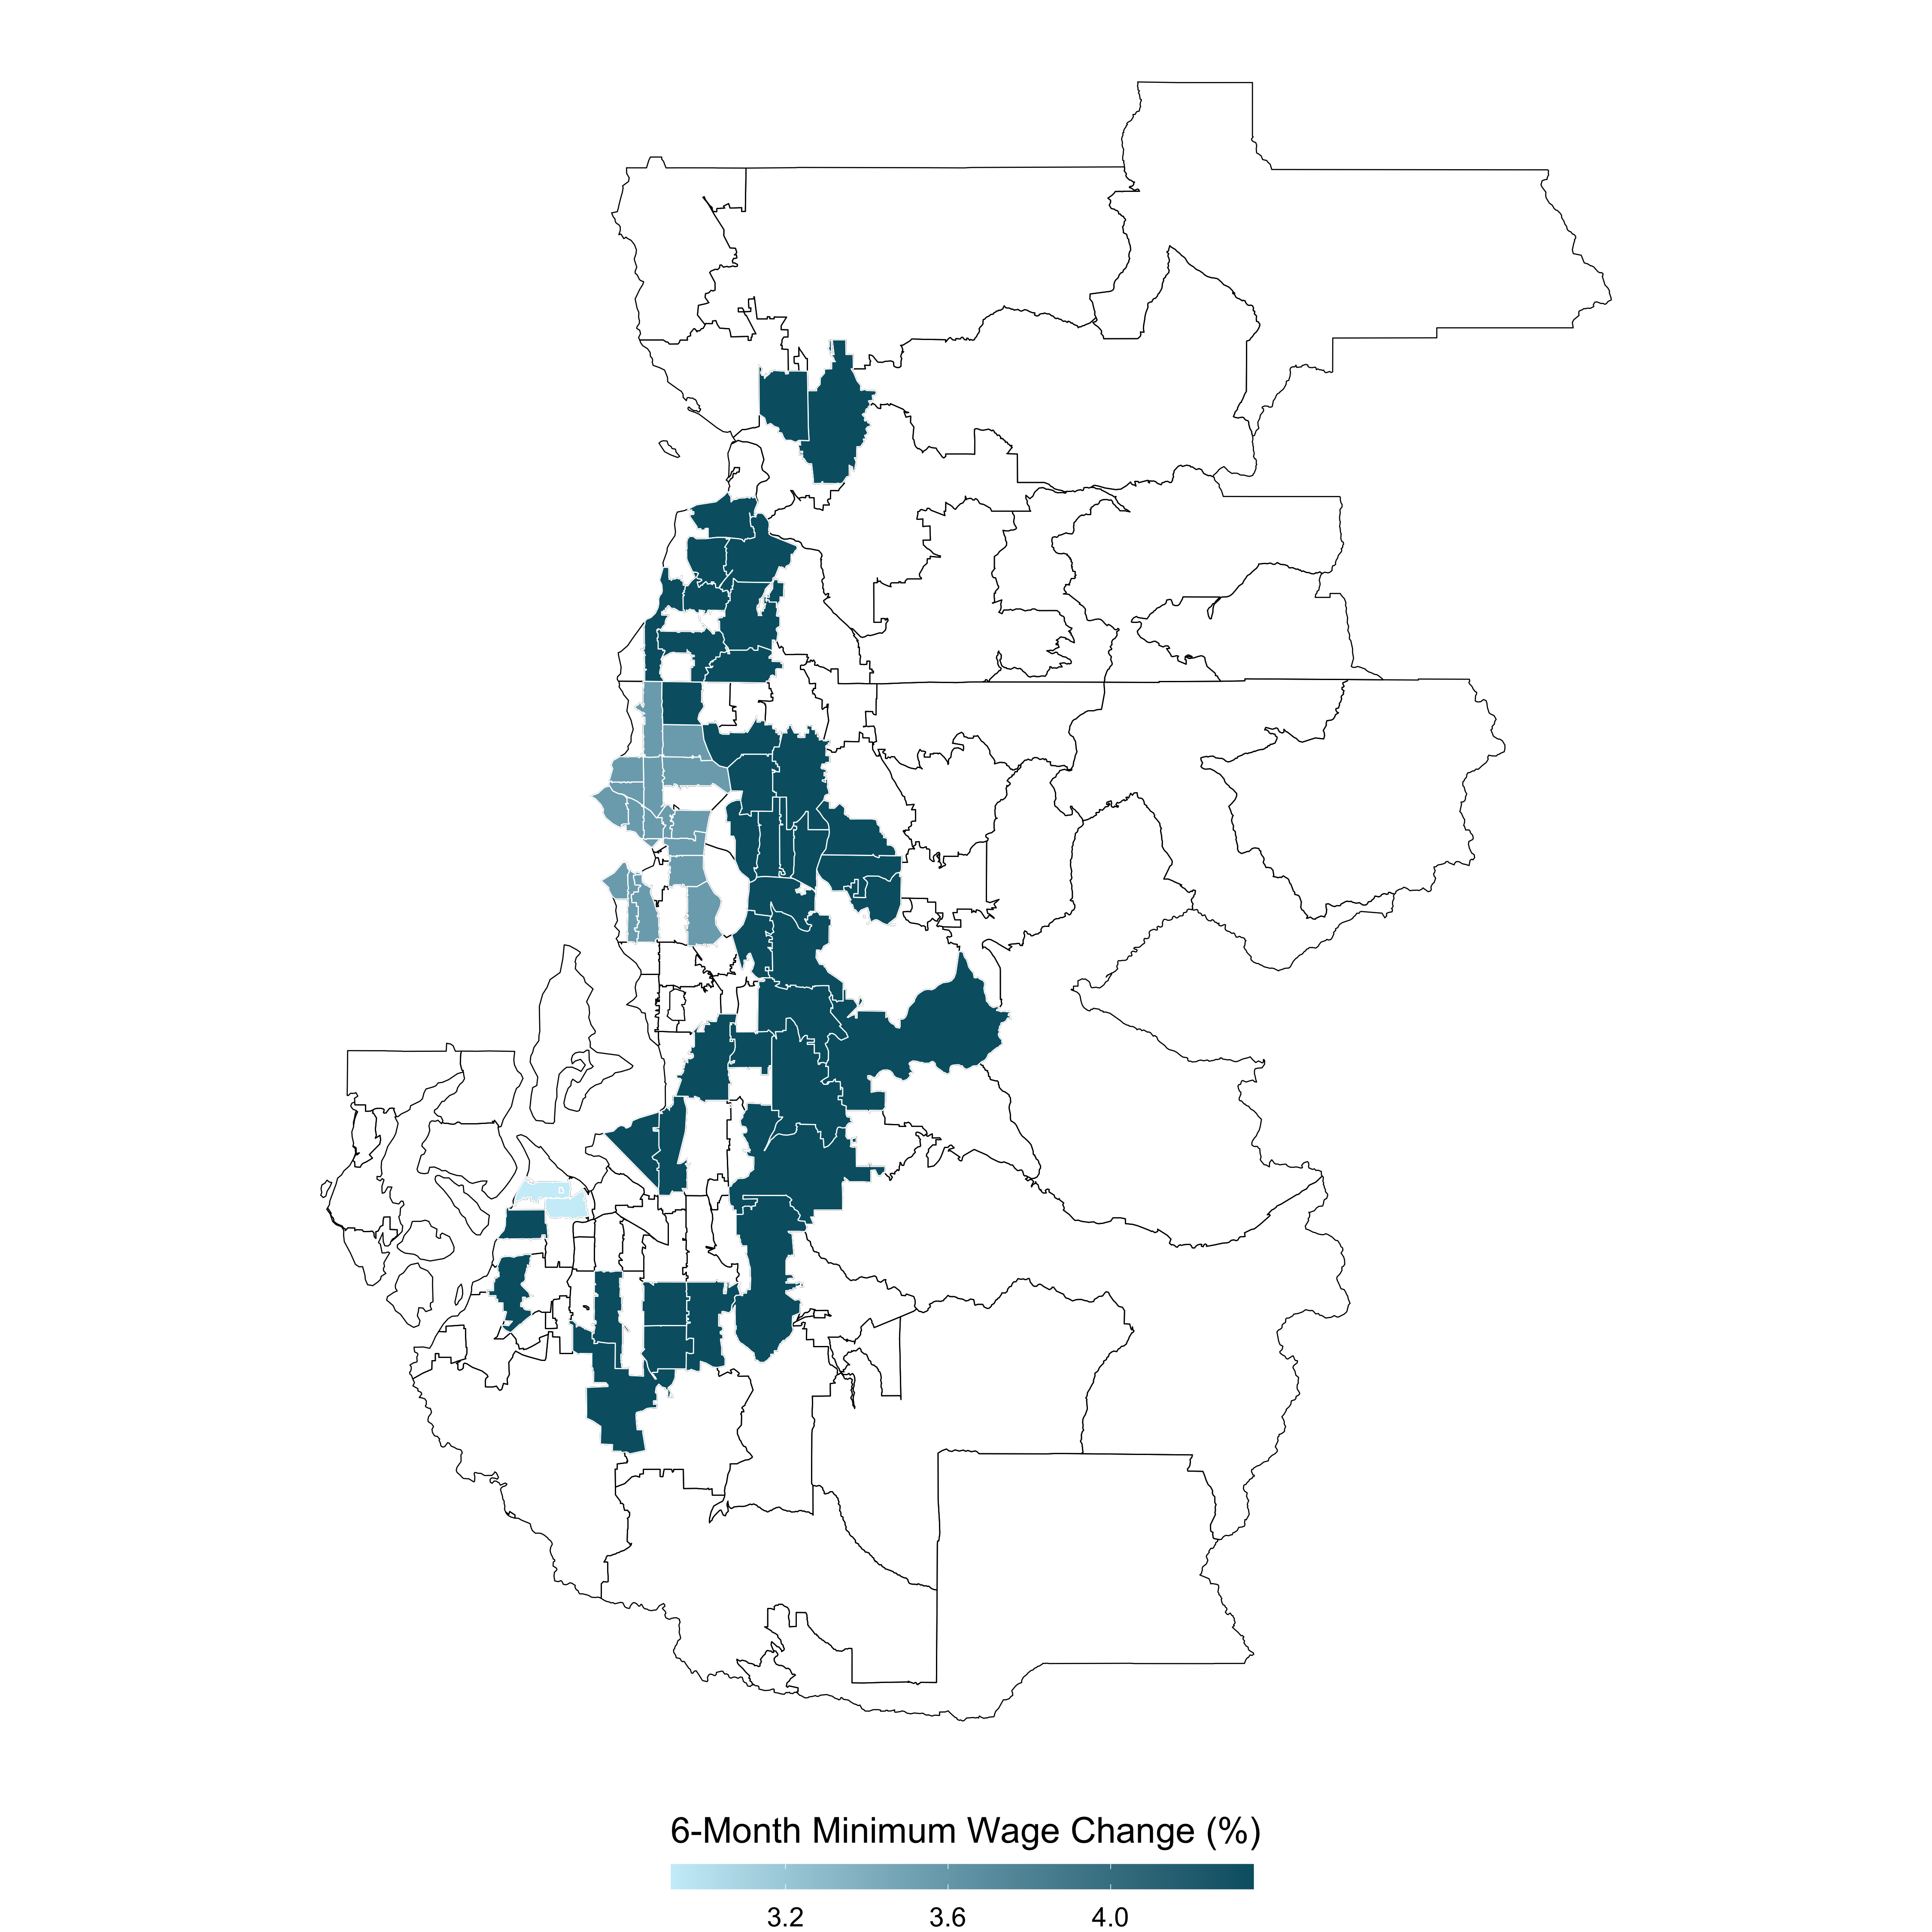
\includegraphics[width = \textwidth]{../../analysis/descriptive_maps/output/Seattle_mw_msa.png}
		\caption{Statutory Minimum Wage}
	\end{subfigure}
	\quad 
	\begin{subfigure}[b]{.8\textwidth}
		\centering
		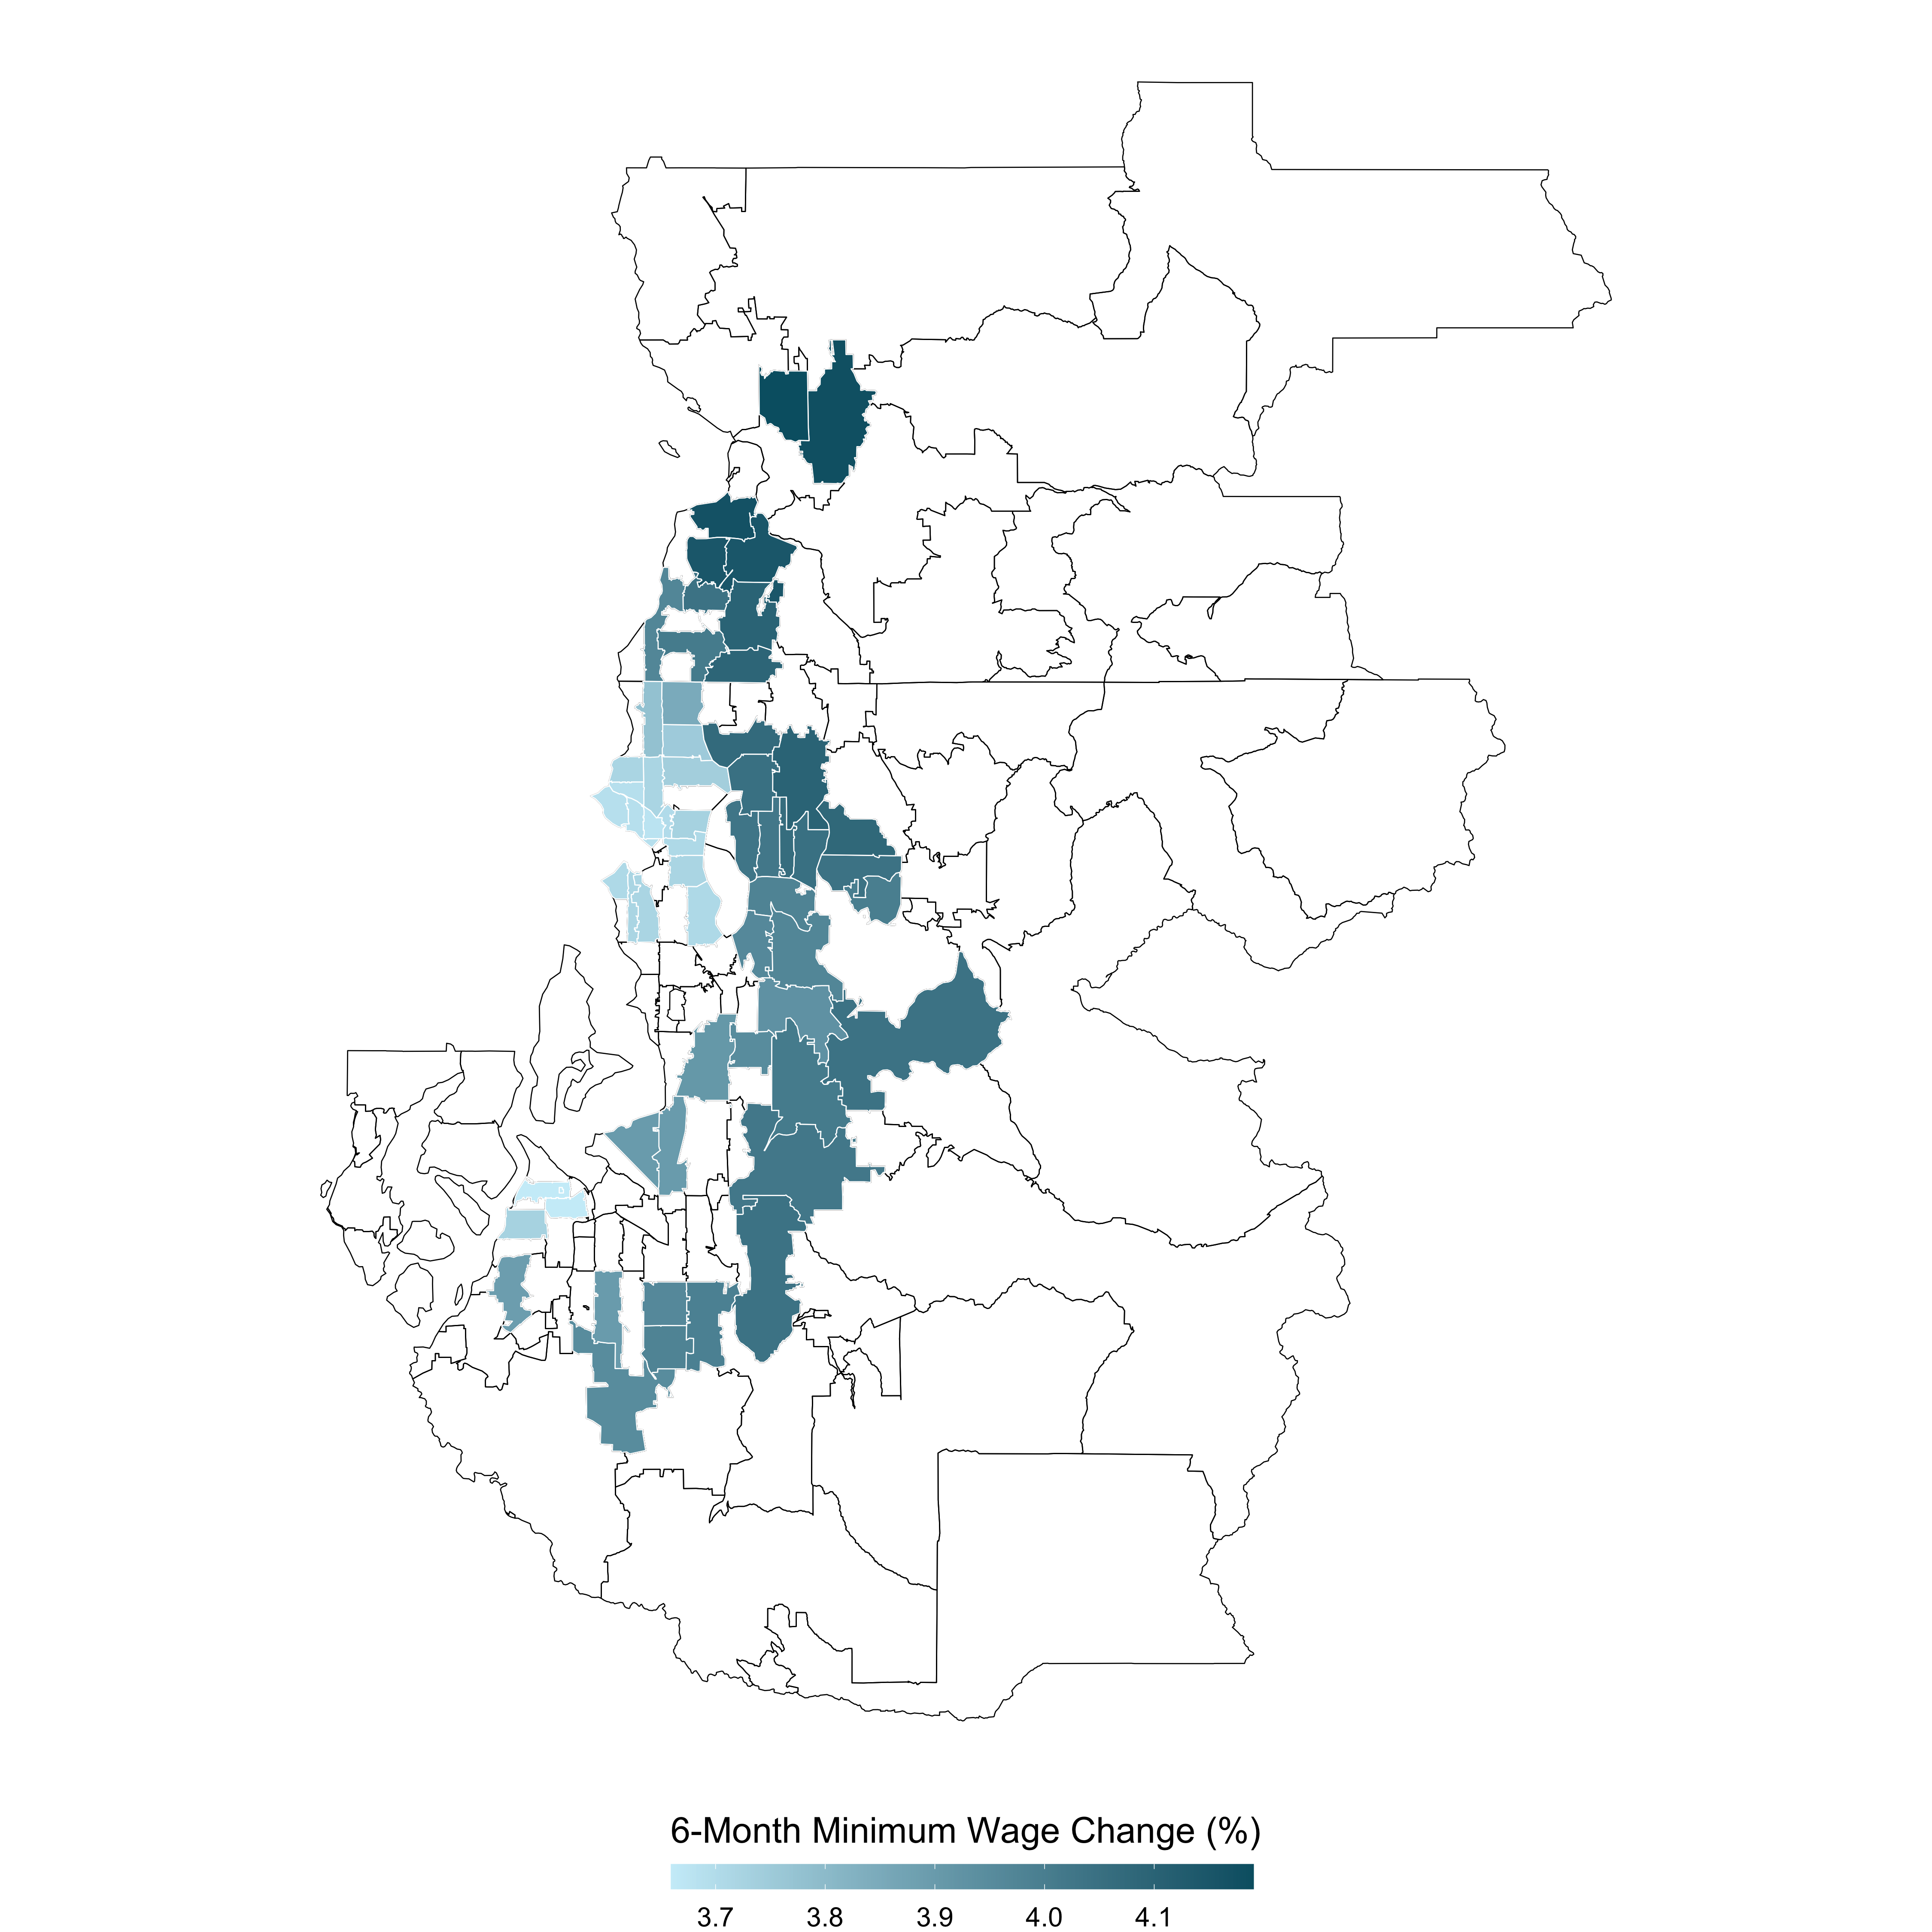
\includegraphics[width = \textwidth]{../../analysis/descriptive_maps/output/Seattle_expmw_msa.png}
		\caption{Experienced Minimum Wage}
	\end{subfigure}
\subcaption*{\textit{Note:} Minimum wage date change: 01 January 2019}
\end{figure}
\end{document}